\documentclass[tikz,border=10pt]{standalone}
\usepackage{amsmath}
\usetikzlibrary{arrows.meta, positioning, calc, fit, decorations.pathreplacing}

\definecolor{c1}{HTML}{000000}  % black       - structure, axes
\definecolor{c2}{HTML}{233D4D}  % deep slate  - the windows we impose, tokens
\definecolor{c3}{HTML}{FE7F2D}  % orange      - the measurements themselves
\definecolor{c4}{HTML}{EAECF0}  % cool grey   - panel fills
\definecolor{axiscolor}{HTML}{333333}
\definecolor{labelcolor}{HTML}{5F6B75}

\begin{document}
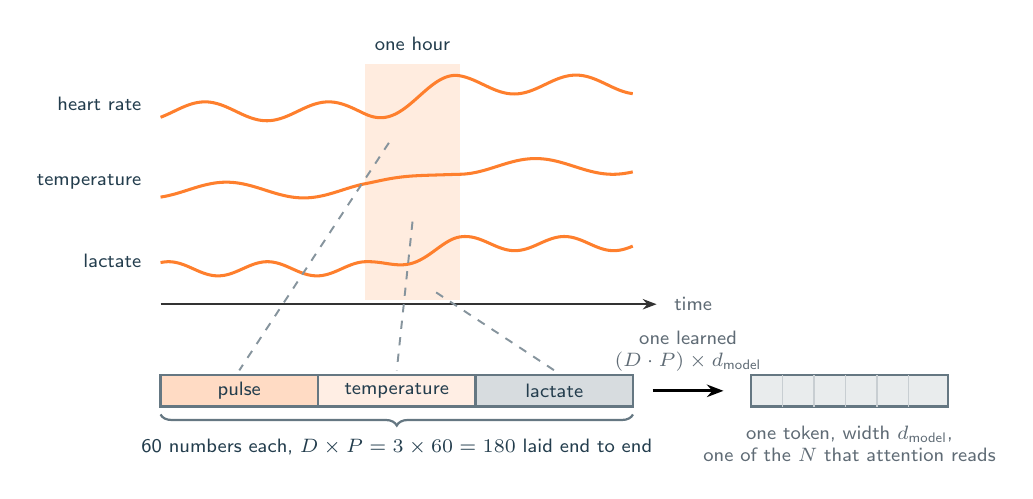
\begin{tikzpicture}[
    every node/.style={font=\sffamily},
    arr/.style={-{Stealth[length=6pt]}, line width=1.1pt, color=c1},
    lab/.style={font=\sffamily\scriptsize, text=labelcolor},
    tag/.style={font=\sffamily\scriptsize, text=c2},
    guide/.style={c2!55, line width=0.7pt, dashed},
    blk/.style={rectangle, draw=c2!70, line width=0.9pt},
]

% ============================================================ the one hour, across all three
\fill[c3!15] (4.00, 3.05) rectangle (5.20, 6.05);
\node[tag, anchor=south] at (4.60, 6.10) {one hour};

% three channels on one clock
\draw[c3, line width=1.1pt]
    plot[domain=1.40:7.40, samples=200, smooth]
    (\x, {5.45 + 0.12*sin(\x r * 4.0) + 0.34*(\x<4.00 ? 0 : (\x>5.20 ? 1 : ((\x-4.00)/1.20)*((\x-4.00)/1.20)*(3-2*((\x-4.00)/1.20))))});
\draw[c3, line width=1.1pt]
    plot[domain=1.40:7.40, samples=200, smooth]
    (\x, {4.45 + 0.10*sin(\x r * 3.2 + 40) + 0.30*(\x<4.00 ? 0 : (\x>5.20 ? 1 : ((\x-4.00)/1.20)*((\x-4.00)/1.20)*(3-2*((\x-4.00)/1.20))))});
\draw[c3, line width=1.1pt]
    plot[domain=1.40:7.40, samples=200, smooth]
    (\x, {3.45 + 0.09*sin(\x r * 5.0 + 20) + 0.32*(\x<4.00 ? 0 : (\x>5.20 ? 1 : ((\x-4.00)/1.20)*((\x-4.00)/1.20)*(3-2*((\x-4.00)/1.20))))});

\node[tag, anchor=east] at (1.28, 5.55) {heart rate};
\node[tag, anchor=east] at (1.28, 4.55) {temperature};
\node[tag, anchor=east] at (1.28, 3.55) {lactate};

\draw[axiscolor, line width=0.8pt, -{Stealth[length=5pt]}] (1.40, 3.00) -- (7.70, 3.00);
\node[lab, anchor=west] at (7.80, 3.00) {time};

% ============================================================ the three windows, laid end to end
\filldraw[blk, fill=c3!28] (1.40, 1.70) rectangle (3.40, 2.10);
\filldraw[blk, fill=c3!13] (3.40, 1.70) rectangle (5.40, 2.10);
\filldraw[blk, fill=c2!18] (5.40, 1.70) rectangle (7.40, 2.10);
\node[tag] at (2.40, 1.90) {pulse};
\node[tag] at (4.40, 1.90) {temperature};
\node[tag] at (6.40, 1.90) {lactate};

\draw[decorate, decoration={brace, amplitude=4pt, mirror}, c2!70, line width=0.8pt]
    (1.40, 1.60) -- (7.40, 1.60)
    node[midway, below=5pt, font=\sffamily\scriptsize, text=c2]
    {60 numbers each, $D \times P = 3 \times 60 = 180$ laid end to end};

% each channel's window drops into its own stretch of that row
\draw[guide] (4.30, 5.05) -- (2.40, 2.16);
\draw[guide] (4.60, 4.05) -- (4.40, 2.16);
\draw[guide] (4.90, 3.15) -- (6.40, 2.16);

% ============================================================ one token
\draw[arr] (7.65, 1.90) -- (8.55, 1.90);
\node[lab, anchor=south, align=center] at (8.10, 2.02)
    {one learned\\ $(D \cdot P) \times d_{\text{model}}$};

\filldraw[blk, fill=c2!10] (8.90, 1.70) rectangle (11.40, 2.10);
\foreach \x in {9.30, 9.70, 10.10, 10.50, 10.90}{
    \draw[c2!25, line width=0.5pt] (\x, 1.70) -- (\x, 2.10);
}
\node[lab, anchor=north, align=center] at (10.15, 1.58)
    {one token, width $d_{\text{model}}$,\\ one of the $N$ that attention reads};

\end{tikzpicture}
\end{document}
